\begin{figure}[!h]
 \centering
 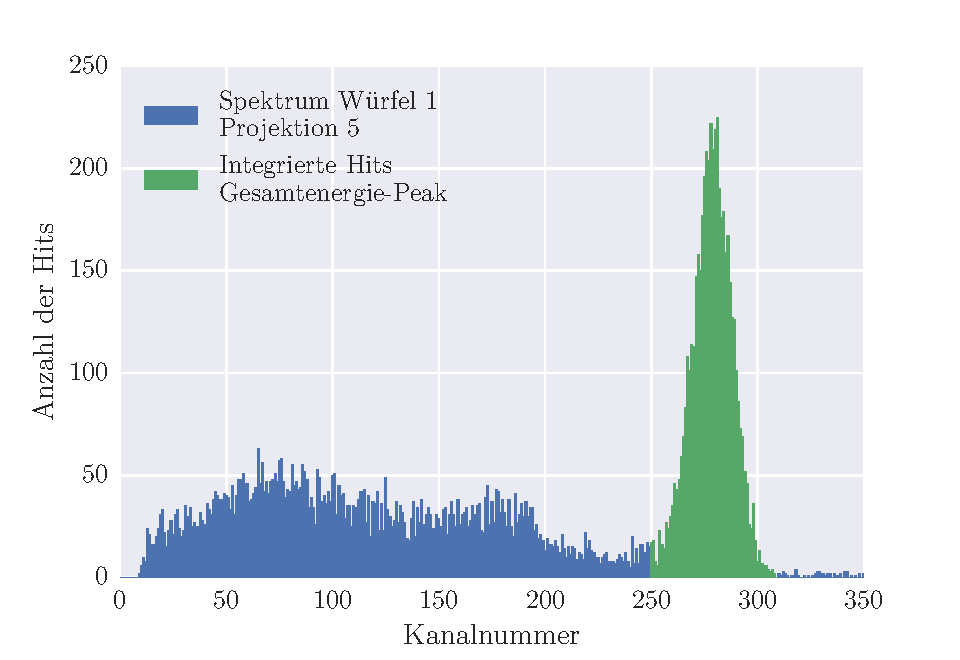
\includegraphics[scale=0.90]{../Grafiken/Spektrum_Block_1_Messung_5_0_350_histogram_intervall.pdf}
 \caption{Beispielhafte Darstellung eines mit dem MCA aufgenommenen 
 	Spektrums. Dabei ist hier nur ein Ausschnitt der 1024 Kanäle gezeigt, da in dem nicht gezeigten Bereich  
 	sehr wenige und nicht relevante Hits aufgenommen wurden. Im speziellen handelt es sich um das Spektrum welche bei der 5. 
 	Projektion der Messung mit Würfel 1 aufgenommen wurde. In grün hervorgehoben ist der Bereich des 
 	Gesamtenergie-Peaks, über den die Anzahl der Hits integriert wurde, um die Materialien der untersuchten 
 	Würfel zu bestimmen.  
 	\label{fig:spektrum_block_1_messung_5_0_350_histogram_intervall}}
 \end{figure} 